
\RequirePackage{fix-cm}
\documentclass[smallextended,natbib]{svjour3}
%% The "natbib" class option makes svjour3 load natbib so that spbasic renders
%% author-year citations (Author Year). Do NOT \usepackage{natbib} again.

\usepackage[T1]{fontenc}
\usepackage{lmodern}

\usepackage{graphicx}
\graphicspath{{figures/}{./}{../figures/}}
\usepackage{multirow}
\usepackage{amsmath,amssymb,amsfonts}
\usepackage{booktabs}
\usepackage{algorithm}
\usepackage{algpseudocode}
\usepackage{tabularx}
\usepackage{makecell}
\usepackage{array}
\newcolumntype{Y}{>{\centering\arraybackslash}X}
\newcolumntype{L}{>{\raggedright\arraybackslash}X}

\usepackage{float}
\usepackage{placeins}
%% Prevent ugly end-of-line hyphenation of these words.
\hyphenation{calibrators Adaptive generalizes effect efficiency
  taxonomies mechanism mechanisms incompatible Poisson Binomial}

%% Discourage (not forbid) line-end word breaks; keep compound words
%% like "pre-trained" whole. \tolerance is raised so lines stay valid.
\tolerance=1500
\hyphenpenalty=4000
\exhyphenpenalty=6000

\journalname{Journal of Combinatorial Optimization}

\begin{document}

\title{Adaptive Poisson--Binomial Joint Conformal Intervals for Reliable Cell
Counting under Distribution Shift}
\titlerunning{Adaptive PB-JCI Online}

%% JOCO uses single-blind review, so real author identities are shown.
\author{Thi Thu Hiep Dinh \and Viet Hang Duong}
\authorrunning{T.T.H. Dinh and V.H. Duong}
\institute{Thi Thu Hiep Dinh \at
           Faculty of Computer Science, University of Information Technology (UIT),
           VNU-HCM, Ho Chi Minh City, Vietnam \\
           ORCID: 0009-0000-8042-3377 \\
           \email{dinhthithuhiep1@gmail.com}
           \and
           Viet Hang Duong (corresponding author) \at
           Faculty of Computer Science, University of Information Technology (UIT),
           VNU-HCM, Ho Chi Minh City, Vietnam \\
           ORCID: 0000-0002-9728-4438 \\
           \email{hangdv@uit.edu.vn}}

\date{Received: date / Accepted: date}

\maketitle

\begin{abstract}
Counting cell nuclei in histopathology images is an important step toward
quantitative biomarkers in computational pathology. However, the counts derived
from current segmentation and detection models are typically point estimates
without uncertainty quantification, a concerning limitation when the deployment
data are distribution-shifted relative to the calibration data. Conformal
prediction yields prediction intervals with coverage guarantees under
exchangeability, but static calibration degrades under shift, while multi-class
counting requires simultaneous coverage of the entire count vector. Adaptive
PB-JCI Online, a lightweight online conformal calibration layer for existing
cell-counting backbones, is proposed. The method models each instance's contribution
with a Poisson--Binomial distribution to obtain an analytic variance scale, uses
a max-statistic across classes to calibrate for joint coverage, and updates the
threshold with a sliding window whose size adapts to recently observed coverage.
On three datasets (PanNuke, NuInsSeg, MoNuSAC) and two backbones (SAM3, PathoSAM),
the max-statistic component attains \(91.7\%\) joint coverage on MoNuSAC with
\(K=4\) classes. Under controlled shift on PanNuke, the method maintains
near-target coverage on SAM3 and substantially improves coverage on PathoSAM,
with prediction intervals narrower than those of adaptive conformal inference. In the cross-dataset shift
PanNuke~\(\to\)~NuInsSeg, where static calibration retains only about \(41\%\)
empirical coverage, the adaptive mechanism restores empirical coverage to
\(90.0 \pm 0.6\%\) and achieves the lowest Winkler score among recent online
conformal baselines.
\keywords{conformal prediction \and uncertainty quantification \and cell counting
\and distribution shift \and Poisson--Binomial \and histopathology}
%% Optional Mathematics Subject Classification (JOCO is a math journal). Fill in
%% suitable MSC2020 codes or delete, e.g.: \subclass{62G08 \and 68T07}
%\subclass{62G08 \and 68T07}
\end{abstract}

%==============================================================================
\section{Introduction}\label{sec:intro}

Counting and classifying cell nuclei in Hematoxylin and Eosin (H\&E)-stained
histopathology images is a fundamental task in digital pathology. Many important
quantitative biomarkers, such as cell density or the ratio between nucleus types,
are derived directly from the number and composition of cells in the tissue.
Recently, foundation models for image segmentation, notably Segment
Anything~\citep{kirillov2023segment} and histopathology-specialized
variants~\citep{archit2025patho}, have substantially reduced annotation costs by
producing instance masks with very little task-specific labeled data. From these
masks, cell counts can be derived by aggregating the detected instances.

However, segmentation-based counting systems typically provide only a point
estimate of the cell count without accompanying uncertainty quantification. This
is an important limitation in biomedical applications, where users need to know
not only how many cells the model predicts, but also how reliable that prediction
is. The problem becomes more serious when the deployment data differ from the
calibration data due to differences in laboratory, staining protocol, scanner, or
tissue type. In such cases, a model with acceptable average error can still
produce overconfident predictions on out-of-domain images.

Conformal prediction~\citep{vovk2005algorithmic, angelopoulos2023gentle} provides
a statistical framework for constructing prediction intervals with finite-sample
coverage guarantees under the assumption of exchangeability between the
calibration and test data. However, applying conformal prediction directly to
multi-class cell counting faces two difficulties. First, static calibrators based
on a fixed calibration set can suffer coverage degradation when the deployment
distribution is shifted~\citep{barber2023conformal, gibbs2021adaptive}. Second, in
the multi-class problem the goal is not only to cover each class individually, but
to cover the entire count vector simultaneously. Calibrating each class
independently, for instance with a Bonferroni
correction~\citep{dunn1961multiple}, can be overly conservative or fail to
directly optimize the joint coverage event.

In this work, Adaptive PB-JCI Online is proposed, an online conformal framework for
multi-class cell counting under distribution shift, built from three components: a
Poisson--Binomial variance scale that normalizes the nonconformity score, a
max-statistic across classes that calibrates joint coverage, and an online
calibration window whose size adapts to recently observed coverage.

The main contributions of this paper are:
\begin{itemize}
\item An analytical uncertainty normalization strategy derived from the
Poisson--Binomial variance is proposed for multi-class counting. By jointly
modeling detection confidence and class uncertainty, the proposed approach
adaptively distributes prediction interval widths in accordance with the
complexity and ambiguity of each image.

\item Prediction intervals with joint coverage for the multi-class count vector
are constructed using a max-statistic across classes, which directly calibrates
the joint coverage event in the split conformal setting under exchangeability.

\item Adaptive PB-JCI Online is introduced, an online conformal calibration
mechanism whose window size adapts to coverage feedback to improve adaptability
when the deployment distribution changes over time.

\item The method is evaluated on three histopathology datasets and two backbones:
the multi-class joint coverage component on PanNuke and MoNuSAC, and the
adaptive-window mechanism in the cross-dataset shift scenario
PanNuke~\(\to\)~NuInsSeg, which is reduced to total cell counting because the
class taxonomies are incompatible.
\end{itemize}

The rest of the paper is organized as follows. Section~\ref{sec:related} reviews
related work; Section~\ref{sec:method} describes the proposed method;
Section~\ref{sec:exp} presents the experimental setup and results; and
Section~\ref{sec:conclusion} concludes.

%==============================================================================
\section{Related Work}\label{sec:related}
%==============================================================================

\textbf{Conformal prediction.}
Conformal prediction~\citep{vovk2005algorithmic} is a statistical framework for
constructing prediction sets or intervals with finite-sample coverage guarantees
under exchangeability. The split (inductive) conformal variant is widely
used for its low cost: a separate calibration set estimates the quantile of the
nonconformity score, which is then applied to test
samples~\citep{angelopoulos2023gentle}. Its guarantee, however, is only marginal
coverage under exchangeability; when the deployment data are shifted, empirical
coverage can degrade substantially.

\textbf{Conformal prediction under distribution shift and in the online setting.}
Several extensions have been proposed to improve conformal prediction when the
exchangeability assumption is violated. Weighted conformal
prediction~\citep{tibshirani2019conformal} adjusts the conformal quantile with
density-ratio weights in the covariate shift setting, but requires a reliable
estimate of this ratio. Adaptive conformal
inference~\citep{gibbs2021adaptive} updates the error level based on coverage
feedback in the online setting, helping prediction intervals adapt as the
distribution changes. Recent developments such as NexCP~\citep{barber2023conformal},
SAOCP~\citep{bhatnagar2023improved}, FACI~\citep{gibbs2024conformal},
COP~\citep{hu2026conformal}, and Rolling-Origin CP~\citep{halkiewicz2026rolling}
continue to study stronger online update mechanisms for non-stationary data. These
provide important baselines, but most target scalar outputs; multi-class counting
instead needs a calibration mechanism for the entire count vector with a per-image,
per-class uncertainty scale.

\textbf{Nuclei segmentation, classification, and counting.}
Nuclei segmentation and classification are important steps in many histopathology
image analysis systems. Datasets such as PanNuke~\citep{gamper2019pannuke},
MoNuSAC~\citep{verma2021monusac}, and
NuInsSeg~\citep{mahbod2024nuinsseg} have advanced research on instance
segmentation, nucleus type classification, and cell counting across many tissues
and organs. These works, including the recent segmentation foundation models, focus
on segmentation, classification, or counting accuracy, and rarely construct
statistically calibrated prediction intervals for cell counts, especially under
distribution shift.

\textbf{Positioning of this work.}
This work adds an uncertainty calibration layer on top of existing backbones; it is
therefore a task-level conformal framework for multi-class cell counting under
distribution shift, not a new segmentation algorithm or conformal guarantee.

%==============================================================================
%% Keep the pipeline figure (defined below) from floating up into Related Work.
\FloatBarrier
\section{Method}\label{sec:method}

For each input image \(x\), the nuclei detector returns \(M\) candidate instances.
For each instance \(i \in \{1,\dots,M\}\), the model provides two quantities: an
objectness score \(s_i \in [0,1]\), reflecting the confidence that the instance is
a valid nucleus, and a class probability distribution \(p_{ik}\) from the type
head, with \(\sum_{k=1}^{K} p_{ik}=1\). In this work, the segmentation and
detection backbones are considered pre-trained or fine-tuned and are kept fixed
throughout the conformal calibration process. The proposed method uses only the
outputs \(\{(s_i,p_{ik})\}_{i=1}^{M}\) to construct prediction intervals for the
count vector \((N_1,\dots,N_K)\), without requiring any update of the backbone
weights. Fig.~\ref{fig:pipeline} gives an overview of the pipeline.

\begin{figure}[!ht]
\centering
\includegraphics[width=\textwidth]{Fig1}
\caption{Overview of the Adaptive PB-JCI Online pipeline, applied online to each
incoming image \(x_t\). A frozen backbone produces per-instance objectness
\(s_i\) and class probabilities \(p_{ik}\); the Poisson--Binomial variance gives a
per-class scale \(\sigma_{t,k}\); and the conformal step builds joint per-class
count intervals \(\mathcal{C}_{t,k}=[\hat N_{t,k}\pm\hat q_t\sigma_{t,k}]\) using
the current threshold \(\hat q_t\). The threshold is the quantile of a buffer
\(\mathcal{B}\) of nonconformity scores, which is warmstarted offline on the
labeled calibration set \(\mathcal{D}_{\mathrm{cal}}\) (passed through the same
pipeline, ``warmstart scores'') and updated online with each new score \(S_t\);
the initial threshold \(\hat q_0\) is \(\hat q_t\) at \(t=1\). After the delayed
true counts \(N_t\) are observed, the coverage indicator \(c_t\) drives an
adaptive window update \(e_{t+1}\) that controls how many recent scores set the
threshold. The red arrow carries \(\hat q_t\) from the calibration buffer to the
conformal step; the black dashed arrow feeds the intervals
\(\mathcal{C}_{t,k}\) into the coverage check}\label{fig:pipeline}
\end{figure}

\subsection{Poisson--Binomial Counting Scores}\label{sec:pb}

For each candidate instance \(i\) and class \(k\), the contribution weight to the
class count is defined as
\begin{equation}
w_{ik}=s_i p_{ik}.
\end{equation}
This weight combines the instance's detection confidence with the corresponding
class probability, and is used as a pragmatic probability that instance \(i\) is a
valid nucleus of class \(k\).

If each instance is viewed as a Bernoulli variable with success probability
\(w_{ik}\), the count of class \(k\) can be written as
\begin{equation}
N_k = \sum_{i=1}^{M} Z_{ik}, \qquad Z_{ik}\sim \mathrm{Bernoulli}(w_{ik}).
\end{equation}
Since the probabilities \(w_{ik}\) can differ across instances, this sum
corresponds to a Poisson--Binomial distribution. Hence, the mean and variance of
the class count are computed in closed form:
\begin{equation}
\hat{N}_k = \mathbb{E}[N_k] = \sum_{i=1}^{M} w_{ik},
\qquad
V_k = \mathrm{Var}[N_k] = \sum_{i=1}^{M} w_{ik}(1-w_{ik}).
\end{equation}

Here \(\hat{N}_k\) serves as the point estimate for the class-\(k\) count, and the
per-class uncertainty scale is defined as
\begin{equation}
\sigma_k = \sqrt{V_k+\varepsilon},
\end{equation}
where \(\varepsilon=10^{-6}\) is a small constant to avoid division by zero when
computing the nonconformity score.

\paragraph{Role of the Poisson--Binomial model.}
The Poisson--Binomial is used as a variance estimator, not as a generative model
for the counts. Its independence assumptions need not hold exactly: detected
instances may be correlated, and the residual deviations after normalization are
absorbed nonparametrically by the conformal threshold on the max-statistic. Thus
\(\sigma_k\) only sets the relative interval width across images and classes, while
coverage is calibrated by the conformal step.

\subsection{Joint Coverage via a Max-Statistic}\label{sec:jci}

Consider a calibration set of \(n_{\mathrm{cal}}\) images, where each image has a
true count vector \((N_1,\dots,N_K)\). For each calibration image, after computing
\(\hat{N}_k\) and \(\sigma_k\), the normalized nonconformity score of class \(k\)
is defined as
\begin{equation}
R_k = \frac{|N_k-\hat{N}_k|}{\sigma_k}.
\end{equation}

To calibrate for the joint coverage event over the entire count vector, a
max-statistic across classes is used:
\begin{equation}
S = \max_{1\leq k\leq K} R_k.
\end{equation}
Instead of constructing a separate threshold for each class, a single threshold is
learned on the nonconformity score \(S\), thereby directly calibrating for the
event that every class is covered.

Let \(S_1,\dots,S_{n_{\mathrm{cal}}}\) be the nonconformity scores on the
calibration set and \(S_{(1)}\leq \cdots \leq S_{(n_{\mathrm{cal}})}\) the sorted
ascending sequence. The split conformal threshold is taken at the index
\begin{equation}
j = \left\lceil (n_{\mathrm{cal}}+1)(1-\alpha) \right\rceil,
\end{equation}
and
\begin{equation}
\hat{q} = S_{(j)}.
\end{equation}
In all experiments, \(n_{\mathrm{cal}} \ge 1/\alpha - 1\) is chosen, so the above
quantile index always lies within the set of calibration points, i.e.
\(j \le n_{\mathrm{cal}}\). Hence, \(\hat q\) is always a finite quantile.

The prediction interval for class \(k\) is constructed on the real line:
\begin{equation}
\mathcal{C}_k
=
\left[
\max\{0,\,\hat{N}_k-\hat{q}\sigma_k\},\;
\hat{N}_k+\hat{q}\sigma_k
\right],
\qquad k=1,\dots,K.
\end{equation}
Here, the lower bound is clipped at 0 to respect the nonnegativity of counts.

Under the assumption that the calibration and test data are exchangeable, applying
split conformal to the nonconformity score \(S\) yields a joint coverage
guarantee:
\begin{equation}
\mathbb{P}\left\{
N_k \in \mathcal{C}_k,\; \forall k=1,\dots,K
\right\}
\geq 1-\alpha.
\end{equation}
When this assumption is violated in online scenarios under distribution shift,
coverage is evaluated empirically.

In the case of only the total cell count, i.e. \(K=1\), \(p_{i1}=1\) and
\(w_{i1}=s_i\). Then \(\hat{N}_1\) and \(\sigma_1\) are computed directly from the
objectness of the detected instances. The max-statistic becomes \(S=R_1\), and the
joint coverage problem reduces to coverage for a single class. Therefore, the
prediction interval for the total cell count can be viewed as a special case of
the proposed calibration framework.

\subsection{Adaptive PB-JCI Online}\label{sec:adaptive}

The static calibration in Section~\ref{sec:jci} uses a fixed threshold \(\hat{q}\)
learned from the initial calibration set. When the deployment distribution
changes, the nonconformity scores in the calibration set may no longer represent
the current data, leading to coverage degradation. Therefore, in the online
setting with label feedback, the conformal threshold is updated using recently
observed nonconformity scores.

At each time \(t\), the method predicts the interval for image \(x_t\) using only
the nonconformity scores in the past buffer. After the prediction is made, the
true count label is observed and the nonconformity score \(S_t\) is added to the
buffer.

The \emph{PB-JCI Online-Fixed} variant uses a fixed window of the \(W\) most recent
nonconformity scores to estimate the threshold at each step. This gradually
discards old calibration points as the distribution changes, but may react slowly
to abrupt or large-magnitude shifts.

The full version, \emph{Adaptive PB-JCI Online}, replaces the fixed window with an
effective window of integer size \(e_t\in\mathbb{Z}_{>0}\) (the number of
nonconformity scores used), adjusted from the coverage observed over the \(m\) most
recent steps. When the average coverage is below the target \(1-\alpha\), the
window is shrunk to adapt faster to the new data domain. When coverage exceeds
\(1-\alpha+\beta\), the window is grown to stabilize the threshold. If coverage
lies within the acceptance region, the window size is kept unchanged. This
mechanism uses only in-stream coverage feedback and does not require an offline
grid search over the window size.
\begin{algorithm}[t]
\caption{Adaptive PB-JCI Online}\label{alg:adaptive}
\begin{algorithmic}[1]
\Require Image stream \(\{x_t\}\); error level \(\alpha\); window bounds \(w_{\min},w_{\max}\);
shrink factor \(\rho_s<1\), grow factor \(\rho_g>1\); coverage window \(m\); dead-band margin \(\beta\)
\State Initialize buffer \(\mathcal{B}\) with the nonconformity scores on the initial calibration set
\State Keep the \(w_{\max}\) most recent points in \(\mathcal{B}\)
\State \(e_1 \gets \min(w_{\max},\lvert\mathcal{B}\rvert)\); \quad \(\mathcal{R}\gets\emptyset\)
\For{each image \(x_t\)}
  \State Compute \(\hat{N}_{t,k}\) and \(\sigma_{t,k}\) as in Section~\ref{sec:pb}
  \State Take the \(e_t\) most recent points from \(\mathcal{B}\) and sort into
  \(S_{(1)}\leq \cdots \leq S_{(e_t)}\)
  \State \(j_t \gets \lceil(e_t+1)(1-\alpha)\rceil\)
  \State \(\hat{q}_t \gets S_{(j_t)}\)
  \State Output the interval
  \[
  \mathcal{C}_{t,k}=
  [\max\{0,\hat{N}_{t,k}-\hat{q}_t\sigma_{t,k}\},\;
   \hat{N}_{t,k}+\hat{q}_t\sigma_{t,k}]
  \]
  for all classes \(k\)
  \State Observe the true counts \(N_{t,k}\)
  \State \(c_t \gets \mathbf{1}\{N_{t,k}\in \mathcal{C}_{t,k},\;\forall k=1,\dots,K\}\)
  \State Append \(c_t\) to \(\mathcal{R}\) and keep the \(m\) most recent values
  \State \(\bar{c}_t \gets \mathrm{mean}(\mathcal{R})\)
  \If{\(\bar{c}_t < 1-\alpha\)}
    \State \(e_{t+1}\gets \max\{w_{\min},\lfloor\rho_s e_t\rfloor\}\)
  \ElsIf{\(\bar{c}_t > 1-\alpha+\beta\)}
    \State \(e_{t+1}\gets \min\{w_{\max},\lfloor\rho_g e_t\rfloor\}\)
  \Else
    \State \(e_{t+1}\gets e_t\)
  \EndIf
  \State \(S_t\gets \max_k \lvert N_{t,k}-\hat{N}_{t,k}\rvert/\sigma_{t,k}\)
  \State Append \(S_t\) to \(\mathcal{B}\) and keep the \(w_{\max}\) most recent points
\EndFor
\end{algorithmic}
\end{algorithm}

Throughout all experiments, the parameters are fixed at \(\alpha=0.1\),
\(w_{\max}=300\), \(w_{\min}=40\), \(m=50\), \(\rho_s=0.9\), \(\rho_g=1.05\), and
\(\beta=0.03\), unless otherwise noted. Since \(w_{\min}\ge 1/\alpha-1\), the
effective window always satisfies \(e_t\ge w_{\min}\), so
\(\lceil(e_t+1)(1-\alpha)\rceil\le e_t\), i.e. the quantile index in
Algorithm~\ref{alg:adaptive} is always valid.

The adaptive mechanism in Algorithm~\ref{alg:adaptive} assumes that the true count
label is observed after the prediction, e.g. through expert review or delayed
annotation. If there is no label feedback during deployment, the system cannot
measure coverage online and therefore cannot update the conformal threshold by the
above mechanism. In that case, distribution shift detectors based on feature
distributions, such as MMD\(^2\), Wasserstein, or Energy distance, can serve as an
alerting signal to trigger offline review and recalibration. These two deployment
regimes are handled by the same calibration layer.

\section{Experiments}\label{sec:exp}

\subsection{Setup}\label{sec:setup}

\textbf{Datasets.}
The method is evaluated on three H\&E-stained nuclei datasets: PanNuke, NuInsSeg,
and MoNuSAC. PanNuke is used as the main dataset for the multi-class counting
experiments with \(K=5\). Following PanNuke's three-fold structure, Fold~1 and
Fold~2 are used to train or fine-tune the predictive components, while Fold~3 is
held out for conformal evaluation. For each calibration seed, the evaluation data
are randomly split \(50/50\) into a calibration set and a test set. The calibration
set is used only to estimate the conformal threshold.

For SAM3, evaluation is performed on all of PanNuke Fold~3, comprising \(2{,}722\)
images with \(n_{\mathrm{cal}}=n_{\mathrm{test}}=1{,}361\) per seed. For PathoSAM,
to avoid potential overlap with the training data, \(494\) colon tissue images are
removed from Fold~3. Specifically, Lizard is one of the PathoSAM training datasets,
aggregating images from multiple colon tissue sources and possibly containing
images from the colon part of PanNuke Fold~3. Therefore, PathoSAM is evaluated on a
subset of \(2{,}228\) images, with
\(n_{\mathrm{cal}}=n_{\mathrm{test}}=1{,}114\) per seed.

NuInsSeg is used for the cross-dataset shift experiment in the total cell counting
problem, i.e. \(K=1\). In this setting, the initial calibration set comes from
PanNuke, while NuInsSeg is treated as a deployment stream to evaluate online
adaptation. MoNuSAC is used to test the generalization of the joint coverage
mechanism in a multi-class counting setting with a different number of classes from
PanNuke, namely \(K=4\). Table~\ref{tab:data_split} summarizes the datasets,
evaluation settings, and nuclei statistics.
\begin{table}[!htbp]
\caption{Summary of datasets, evaluation settings, and nuclei statistics. For
PanNuke Fold-3, the \#Images/\#Nuclei columns correspond to the \(2{,}228\)-image
subset used for PathoSAM (after removing \(494\) colon images); SAM3 is evaluated
on all \(2{,}722\) Fold-3 images}
\label{tab:data_split}
\centering
\small
\setlength{\tabcolsep}{4pt}
\begin{tabularx}{\textwidth}{@{}LlclLcc@{}}
\toprule
Dataset & Task & \(K\) & Train & Cal/Test & \#Images & \#Nuclei \\
\midrule
PanNuke (Fold-3, subset) & multi-class counting & 5 & Fold~1+2 & Fold~3 (\(50/50\)) & \(2{,}228\) & \(54{,}835\) \\
NuInsSeg & total counting & 1 & - & PanNuke cal \(\to\) stream & \(665\) & \(35{,}138\) \\
MoNuSAC (test) & multi-class counting & 4 & train split & cal/test split & \(96\) & \(15{,}997\) \\
\bottomrule
\end{tabularx}
\end{table}

\textbf{Predictors and type head.}
Two different segmentation and detection backbones are used to test how much the
conformal calibration layer depends on the predictive architecture. The first
backbone is SAM3~\citep{carion2025sam3}, fine-tuned with LoRA~\citep{hu2022lora} on
the decoder; the second backbone is PathoSAM~\citep{archit2025patho}, a model
specialized for nuclei segmentation in histopathology images. After the initial
training or fine-tuning stage, the backbones are kept fixed throughout the
conformal experiments.

For each detected instance the backbone provides an objectness score \(s_i\); a type
head applied to the mask-pooled instance feature yields the class probability
\(p_{ik}\). It is a two-layer MLP with a softmax over \(K\) classes, trained with
class-weighted cross-entropy and then kept fixed. The conformal layer uses only
\((s_i,p_{ik})\) and the count labels on the calibration set.

\textbf{Distribution-shift scenarios.}
Four controlled shift scenarios are evaluated on PanNuke: in-distribution, mild
shift, severe shift, and temporal distribution drift. In the in-distribution
scenario, the test data share the same domain as the calibration set. Color and
morphological image transformations including HED, HSV jitter, and Gaussian blur
are studied at multiple intensities; in the main experiments, the mild shift
level is represented by HSV jitter, and the severe shift level by Gaussian blur. In
the drift scenario, the test stream is ordered by increasing shift magnitude, from
in-distribution to mild and severe, to simulate a distribution changing over time.

The shift magnitude of the transformations is quantified by MMD\(^2\),
Wasserstein-1, and Energy distance in Appendix~\ref{secA:shift}. The results show
that the feature deviation increases with the transformation intensity, while the
difference between PanNuke folds is very small.

\textbf{Baselines.}
\emph{Marginal Split} calibrates each class at level \(\alpha\), guaranteeing only
marginal coverage for each class without calibrating for joint coverage.
\emph{PB-JCI Split} is the static version of the proposed method, using the
Poisson--Binomial scale and the max-statistic but keeping the conformal threshold
fixed. \emph{PB-JCI Online-Fixed} uses the same joint nonconformity score but
updates the threshold with a fixed sliding window. \emph{Class-Strat Bonferroni}
calibrates each class separately with an error level allocated by the Bonferroni
correction. In the cross-dataset scenario, modern online conformal methods including
ACI, NexCP, FACI, SAOCP, COP, and Rolling-Origin CP are additionally compared.

Unless otherwise noted, all online methods are initialized from the same initial
calibration buffer, process the same data stream order, and receive label feedback
after prediction at the same time. This setup attributes the differences in results
mainly to the calibration mechanism rather than to the amount of information used.
The threshold update rules of the online conformal baselines are summarized in
Appendix~\ref{secA:baselines}.

\textbf{Metrics.}
The main metric is joint coverage. For image \(t\), the prediction is considered
covered if \(N_{t,k}\in \mathcal{C}_{t,k}\) for all classes \(k=1,\dots,K\).
Coverage is computed as the fraction of images satisfying this condition. The
average width is also reported, computed as the mean interval width over classes
and over images. Since the average width can be dominated by a few very wide
intervals, in the cross-dataset shift scenario, where the width distribution is
strongly skewed, the median width is additionally reported as a more robust measure
of the typical width. In the \(K=1\) problem, the width corresponds to the prediction interval
width for the total cell count.

Beyond coverage and width, the Winkler score, also known as the interval
score~\citep{winkler1972decision}, is used to jointly assess the narrowness and
reliability of the prediction interval:
\begin{equation}
\mathrm{WS}_{\alpha}(\ell,u;y)
=
(u-\ell)
+
\frac{2}{\alpha}(\ell-y)\mathbf{1}\{y<\ell\}
+
\frac{2}{\alpha}(y-u)\mathbf{1}\{y>u\}.
\end{equation}
The Winkler score equals the width when the true value lies inside the interval and
adds a penalty otherwise, so a lower score indicates a better balance between
coverage and width. All three metrics are aggregated as mean \(\pm\) standard
deviation across seeds.

In the online experiments, local coverage and local width are additionally reported
over a sliding window \(W_\ell=50\) to analyze the dynamics around the shift point.

\textbf{Implementation details.}
Each configuration is run with multiple calibration seeds or stream seeds, as noted
in each results table. For SAM3, the mean and standard deviation are reported over
15 runs, comprising 3 model seeds and 5 calibration seeds; for PathoSAM, results are
reported over 5 calibration seeds. In the cross-dataset experiment, the online
methods are evaluated over 5 stream seeds. The tables report mean \(\pm\) standard
deviation, except for deterministic baselines that do not depend on the stream
order. Training hyperparameters and conformal configuration details are listed in
Appendix~\ref{secA:impl}.

\textbf{Evaluation design.}
The experimental design separates the two roles of the framework. Joint coverage
(the Poisson--Binomial scale with the max-statistic) is evaluated on datasets with
a defined taxonomy, PanNuke and MoNuSAC. The adaptive-window mechanism targets
severe online shift and is evaluated in the cross-dataset scenario
PanNuke~\(\to\)~NuInsSeg, reduced to total cell counting (\(K=1\)) because the
taxonomies are incompatible; on the within-dataset PanNuke shifts, PB-JCI
Online-Fixed isolates the sliding-window effect.

\subsection{Conformal Counting under Controlled Shift}\label{sec:main}

Table~\ref{tab:main} evaluates joint conformal counting under four controlled shift
regimes on PanNuke, examining whether PB-JCI attains the in-distribution target, how
much static calibration degrades as the shift grows, and whether the trend holds
across both backbones, SAM3 and PathoSAM.

\begin{table}[!htbp]
\caption{Joint conformal counting under controlled shift on two backbones.
Each cell reports Coverage~\% (top) and Width (bottom) as mean \(\pm\) standard
deviation; the target coverage is 90\%. Bold rows mark the proposed variant (PB-JCI
Online-Fixed), not necessarily the best result}
\label{tab:main}
\centering
\scriptsize
\setlength{\tabcolsep}{2.5pt}
\renewcommand{\arraystretch}{1.15}
\begin{tabularx}{\textwidth}{@{}p{0.23\textwidth}YYYY@{}}
\toprule
Method & In-dist & Mild & Severe & Drift \\
\midrule
\multicolumn{5}{@{}l}{\textit{(a) Backbone: SAM3 (LoRA)}}\\[2pt]
Marginal Split
& \makecell{62.7$\pm$1.6\\9.63$\pm$0.57}
& \makecell{54.8$\pm$1.9\\10.01$\pm$0.62}
& \makecell{61.8$\pm$2.0\\9.19$\pm$0.41}
& \makecell{59.9$\pm$1.5\\9.60$\pm$0.54} \\

ACI
& \makecell{89.9$\pm$0.1\\14.62$\pm$0.79}
& \makecell{89.7$\pm$0.1\\18.70$\pm$1.41}
& \makecell{89.3$\pm$0.2\\24.54$\pm$1.42}
& \makecell{89.4$\pm$0.1\\19.45$\pm$1.24} \\

PB-JCI Split
& \makecell{90.0$\pm$1.3\\13.54$\pm$0.74}
& \makecell{82.9$\pm$1.2\\13.93$\pm$0.80}
& \makecell{81.1$\pm$2.2\\12.79$\pm$0.53}
& \makecell{84.8$\pm$1.0\\13.41$\pm$0.70} \\

\textbf{PB-JCI Online-Fixed}
& \makecell{\textbf{90.5$\pm$0.3}\\\textbf{13.76$\pm$0.74}}
& \makecell{\textbf{89.9$\pm$0.3}\\\textbf{16.18$\pm$0.88}}
& \makecell{\textbf{89.4$\pm$0.4}\\\textbf{17.77$\pm$0.34}}
& \makecell{\textbf{89.3$\pm$0.4}\\\textbf{15.56$\pm$0.59}} \\

Class-Strat Bonferroni
& \makecell{94.4$\pm$1.1\\18.59$\pm$0.69}
& \makecell{89.2$\pm$1.5\\19.05$\pm$0.78}
& \makecell{85.3$\pm$1.8\\16.19$\pm$0.41}
& \makecell{89.9$\pm$1.1\\17.91$\pm$0.62} \\
\midrule
\multicolumn{5}{@{}l}{\textit{(b) Backbone: PathoSAM}}\\[2pt]
Marginal Split
& \makecell{65.1$\pm$1.9\\8.84$\pm$0.14}
& \makecell{57.6$\pm$1.8\\8.93$\pm$0.13}
& \makecell{17.3$\pm$0.7\\6.98$\pm$0.09}
& \makecell{46.4$\pm$1.2\\8.28$\pm$0.16} \\

ACI
& \makecell{89.9$\pm$0.1\\14.79$\pm$0.58}
& \makecell{89.6$\pm$0.1\\18.05$\pm$0.57}
& \makecell{87.4$\pm$0.3\\68.70$\pm$2.36}
& \makecell{87.2$\pm$0.3\\32.76$\pm$1.64} \\

PB-JCI Split
& \makecell{89.7$\pm$1.0\\13.67$\pm$0.19}
& \makecell{83.8$\pm$1.3\\13.75$\pm$0.22}
& \makecell{35.7$\pm$1.2\\11.38$\pm$0.17}
& \makecell{70.1$\pm$1.1\\12.98$\pm$0.24} \\

\textbf{PB-JCI Online-Fixed}
& \makecell{\textbf{90.4$\pm$0.2}\\\textbf{13.94$\pm$0.33}}
& \makecell{\textbf{89.2$\pm$0.4}\\\textbf{15.87$\pm$0.13}}
& \makecell{\textbf{85.7$\pm$0.4}\\\textbf{54.02$\pm$0.52}}
& \makecell{\textbf{85.6$\pm$0.5}\\\textbf{23.87$\pm$0.45}} \\

Class-Strat Bonferroni
& \makecell{96.6$\pm$0.5\\20.17$\pm$0.64}
& \makecell{93.7$\pm$0.7\\20.20$\pm$0.66}
& \makecell{48.5$\pm$1.7\\16.54$\pm$0.73}
& \makecell{79.6$\pm$0.8\\19.05$\pm$0.68} \\
\bottomrule
\end{tabularx}
\end{table}

On SAM3 (block a), static calibration is insufficient under shift: Marginal Split
attains only \(54.8\)--\(62.7\%\) coverage, while PB-JCI Split degrades from
\(90.0\%\) in-distribution to \(81.1\%\) in the severe regime. ACI maintains
near-target coverage \((\approx 89\%)\) but its width increases sharply, reaching
\(24.54\) in the severe regime. In contrast, PB-JCI Online-Fixed keeps coverage
around \(89\)--\(90\%\) in all regimes and produces markedly narrower intervals than
ACI; in the severe regime, the width decreases from \(24.54\) to \(17.77\), about
\(28\%\) narrower. Class-Strat Bonferroni tends to over-cover and produce wide
intervals, revealing the drawback of calibrating each class independently.

A similar improvement trend appears on PathoSAM (block b), a backbone different from
SAM3. PB-JCI Split degrades sharply under severe shift, retaining only \(35.7\%\)
coverage, while PB-JCI Online-Fixed raises coverage to \(85.7\%\) and still produces
narrower intervals than ACI (\(54.02\) versus \(68.70\)). However, because PathoSAM
tends to be overconfident, leading to small \(\sigma_k\), the fixed window does not
fully restore coverage in the severe scenario. This trend holds across both
backbones and motivates the full version Adaptive PB-JCI Online, evaluated in
Section~\ref{sec:cross}.

\subsection{Cross-Dataset Shift and Online Conformal Baselines}\label{sec:cross}

A cross-dataset shift scenario is evaluated with the PathoSAM backbone, calibrating
on PanNuke and deploying on NuInsSeg. This is harder than the controlled shifts of
Section~\ref{sec:main}, since source and target differ in dataset, organ, annotation
protocol, and imaging characteristics. The problem is aggregated to total cell
counting (\(K=1\)), so every online baseline processes the same sequence of scalar
scores from the same PanNuke buffer with the same label feedback.

\begin{table}[!ht]
\caption{Cross-dataset shift with PathoSAM in the PanNuke $\to$ NuInsSeg setting.
The target coverage is $90\%$; coverage and Winkler are reported as mean $\pm$
standard deviation over 5 stream seeds. Lower Winkler is better}
\label{tab:cross}
\centering
\begin{tabular}{@{}lcccc@{}}
\toprule
Method & Coverage (\%) & Avg. width & Med. width & Winkler $\downarrow$ \\
\midrule
ACI
& 84.0$\pm$0.2 & 63.58 & 50.50 & 129.55$\pm$3.78 \\
NexCP
& 84.7$\pm$0.6 & 55.52 & 50.84 & 119.56$\pm$1.29 \\
FACI
& 85.1$\pm$0.6 & 56.71 & 51.28 & 118.93$\pm$0.99 \\
SAOCP
& 87.8$\pm$0.5 & 61.32 & 54.70 & 113.63$\pm$1.53 \\
COP
& 87.9$\pm$0.2 & 60.60 & 54.91 & 113.13$\pm$2.00 \\
Rolling-Origin CP
& 89.5$\pm$0.7 & 64.39 & 58.19 & 110.24$\pm$2.54 \\
PB-JCI Online-Fixed
& 81.8$\pm$1.0 & 53.11 & 47.75 & 125.96$\pm$2.17 \\
\textbf{Adaptive PB-JCI Online}
& \textbf{90.0$\pm$0.6} & 66.50 & 60.02 & \textbf{108.67$\pm$2.94} \\
\bottomrule
\end{tabular}
\end{table}

The static and semi-adaptive methods all fall short of the target
(Table~\ref{tab:cross}). PB-JCI Online-Fixed attains only $81.8\pm1.0\%$, as its
fixed window reacts too slowly; ACI, NexCP, and FACI reach $84$--$85\%$, while SAOCP,
COP, and Rolling-Origin CP come closer at $87.8$--$89.5\%$.

Adaptive PB-JCI Online is the only method that reaches the nominal level
($90.0\pm0.6\%$) and attains the lowest Winkler score ($108.67\pm2.94$). Its
contribution is recovering coverage under shift rather than narrowing intervals:
the larger average width ($66.50$) reflects the trade-off accepted to restore
coverage for an out-of-domain, overconfident predictor, while the median width
($60.02$) stays close to Rolling-Origin CP ($58.19$), showing that the increase
comes mainly from a few hard images.

Fig.~\ref{fig:streaming} illustrates these dynamics: after the domain-change point
the local coverage of the static methods drops, while Adaptive PB-JCI Online adjusts
the threshold to restore local coverage near the target, at the cost of wider
intervals in the hard-data region.

\begin{figure}[!htbp]
\centering
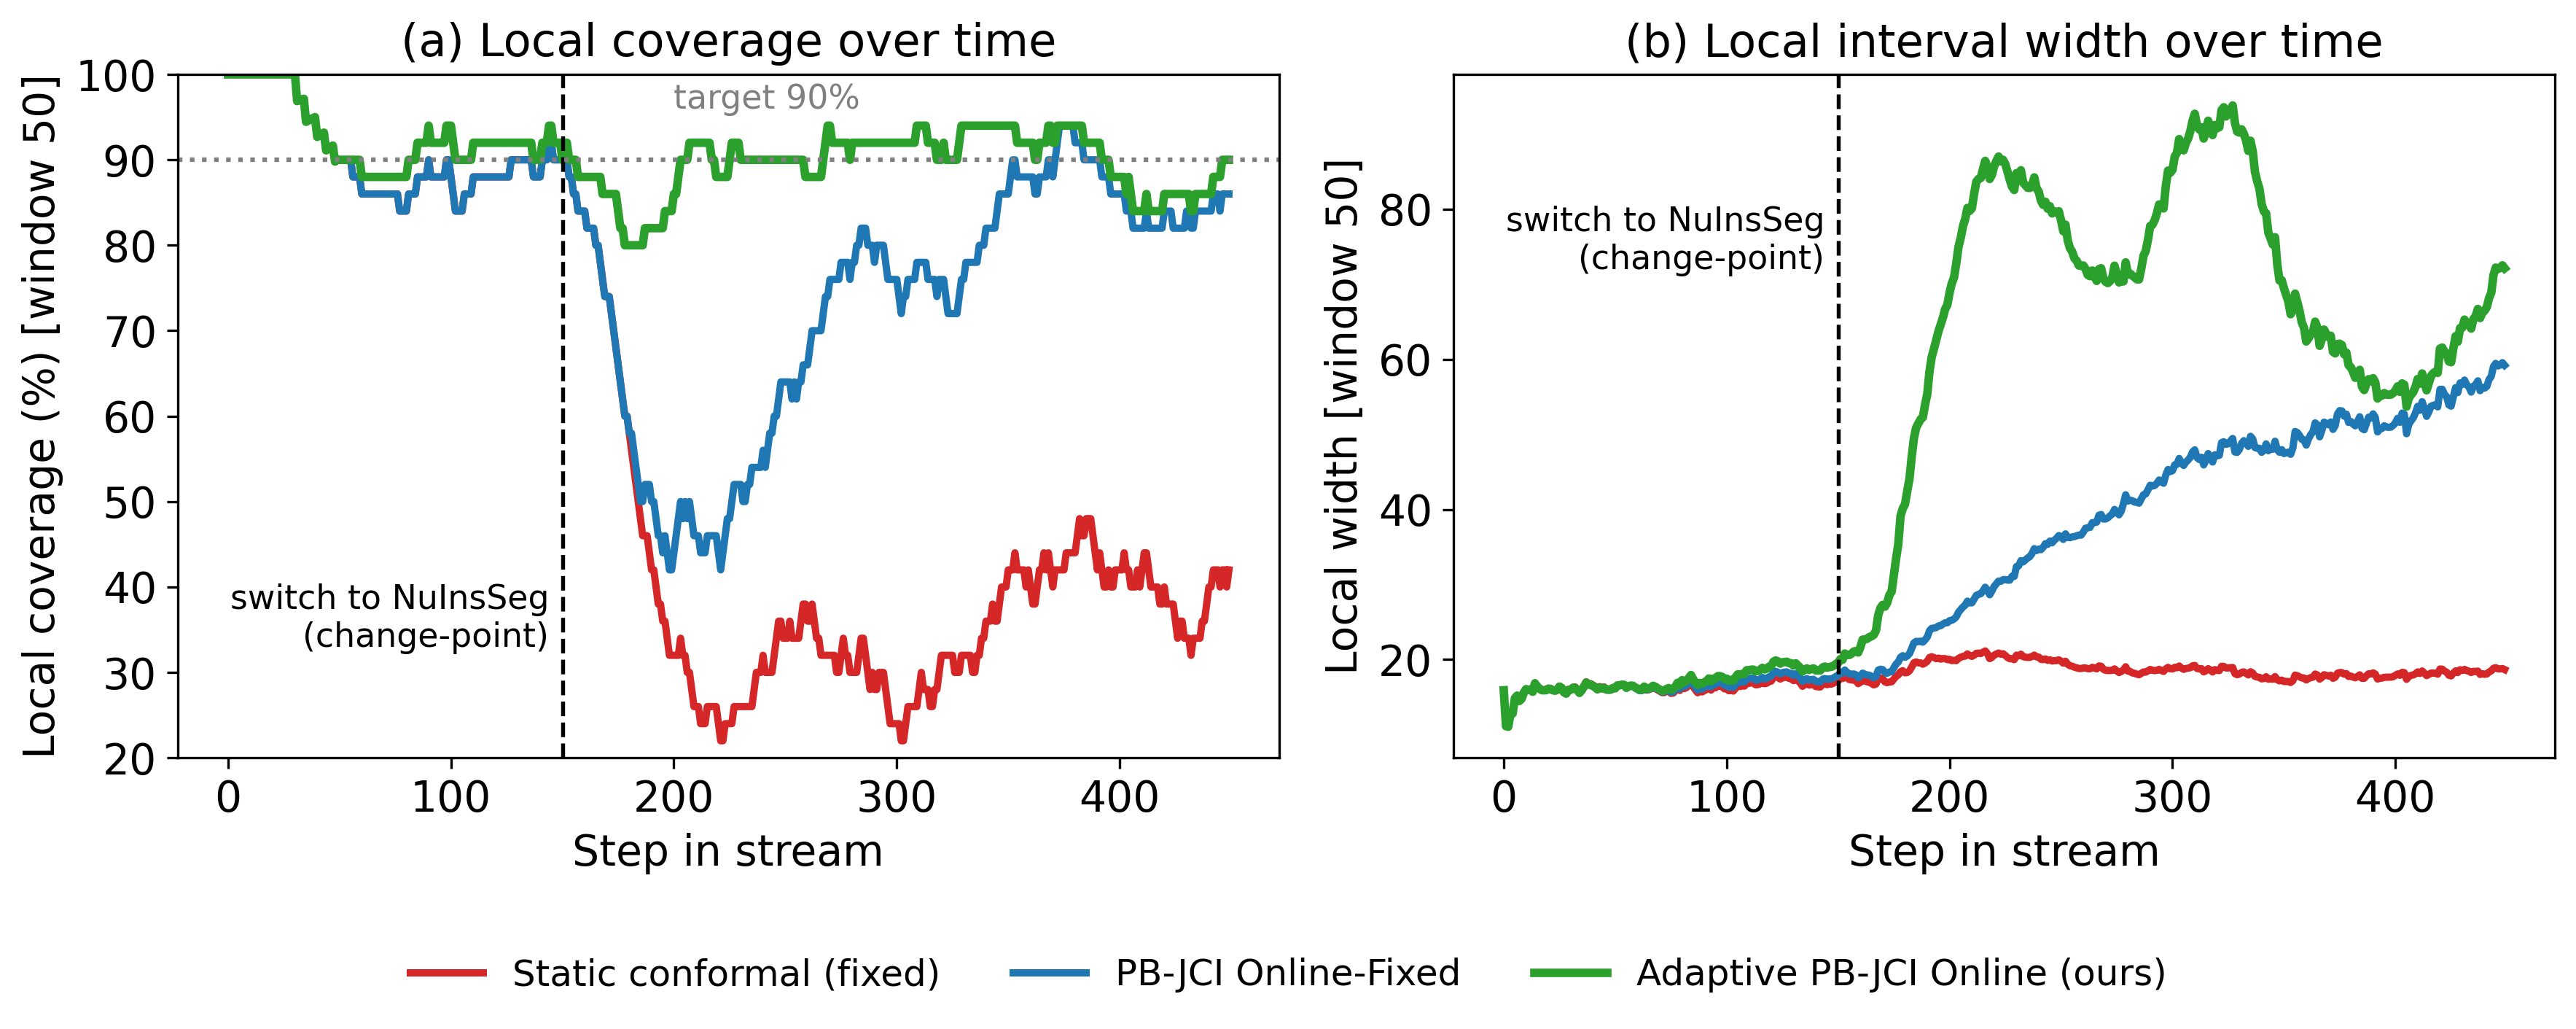
\includegraphics[width=\textwidth]{Fig2.png}
\caption{Online dynamics under cross-dataset shift PanNuke $\to$ NuInsSeg with the
PathoSAM backbone. Quantities are computed over a sliding window of 50 steps:
\textbf{(a)} local coverage versus the 90\% target; \textbf{(b)} local width}
\label{fig:streaming}
\end{figure}

\subsection{Ablation Study}\label{sec:ablation}

A leave-one-out ablation is conducted on the cross-dataset scenario PathoSAM:
PanNuke~\(\to\)~NuInsSeg, whose large discrepancy clarifies each component's
contribution. Since NuInsSeg is single-class \((K=1)\), the ablation covers the
conformal layer, the Poisson--Binomial scale, and the adaptive window; the
max-statistic is evaluated separately at the end of this section.

\begin{table}[!htbp]
\caption{Leave-one-out ablation with target coverage $90\%$.
Each variant removes one component from the full model. Lower Winkler is better}
\label{tab:ablation}
\centering
\small
\begin{tabular}{@{}lccc@{}}
\toprule
Variant & Coverage (\%) & Avg.\ width & Winkler $\downarrow$ \\
\midrule
Naive PB interval, no conformal       & $10.4$        & $4.19$  & $319.09$ \\
Full w/o online update (static split) & $41.5$        & $18.00$ & $226.44$ \\
Full w/o adaptive window (fixed)      & $81.8\pm1.0$  & $53.11$ & $125.96\pm2.17$ \\
Full w/o PB-$\sigma$ (raw residual)   & $90.0\pm0.5$  & $83.47$ & $156.37\pm2.08$ \\
\midrule
\textbf{Full Adaptive PB-JCI Online}  & $\mathbf{90.0\pm0.6}$ & $66.50$ & $\mathbf{108.67\pm2.94}$ \\
\bottomrule
\end{tabular}
\end{table}

Table~\ref{tab:ablation} shows that each component plays a distinct role in the
system. When the entire conformal layer is removed and only intervals based on the
Poisson--Binomial variance are used, the Naive PB interval variant attains only $10.4\%$
coverage despite a very small average width $(4.19)$. This result shows that the
analytic variance provides only an initial uncertainty scale, insufficient to
produce reliable prediction intervals; the actual deviation level still needs to be
calibrated by conformal calibration.

Online updating is the key factor under cross-dataset shift. When the full method is
replaced by static split conformal, coverage attains only $41.5\%$, showing that the
threshold learned from the PanNuke source domain no longer fits the NuInsSeg target
domain. Using a fixed online window improves coverage to $81.8\pm1.0\%$, but still
does not reach the target because the fixed window reacts slowly to strong shift. In
contrast, the adaptive-window mechanism restores the average coverage to
$90.0\pm0.6\%$, showing that adjusting the window size based on coverage feedback is
necessary in this setting.

The PB-\(\sigma\) scale mainly affects the efficiency of the prediction interval
rather than the ability to attain coverage. When PB-\(\sigma\) is removed and the
raw residual is used, the method still attains $90.0\pm0.5\%$ coverage thanks to the
adaptive online mechanism, but the average width increases from $66.50$ to $83.47$,
and the Winkler increases from $108.67$ to $156.37$. This shows that the
Poisson--Binomial variance helps allocate width according to the difficulty of each
image, rather than having to widen intervals almost uniformly to compensate for the
hard cases.

Since NuInsSeg is single-class \((K=1)\), the max-statistic coincides with the
scalar score and is not tested here; it is evaluated separately on multi-class data.
On PanNuke in-distribution (Table~\ref{tab:main}), the max-statistic attains
$90.4\%$ coverage at width $13.94$, whereas per-class Bonferroni over-covers
($96.6\%$) at width $20.17$, confirming that the max-statistic calibrates the joint
event without the conservativeness of independent per-class calibration. Its
generalization to a different number of classes is examined on MoNuSAC \((K=4)\) in
Section~\ref{sec:monusac}.

\subsection{Generalization to a Different Number of Classes}\label{sec:monusac}

The main experiments on PanNuke use \(K=5\) classes, while the cross-dataset
experiment on NuInsSeg is reduced to a single-class problem \((K=1)\). To assess
whether the max-statistic-based joint coverage mechanism depends on the specific
number of classes in PanNuke, an additional experiment is conducted on MoNuSAC, a
dataset with \(K=4\) nucleus classes. This setting tests the generalization of
PB-JCI in a multi-class counting problem with a different label structure.

\begin{table}[!htbp]
\caption{Generalization to a different number of classes on MoNuSAC (\(K=4\), target
joint coverage \(90\%\))}
\label{tab:monusac}
\centering
\begin{tabular}{@{}lcc@{}}
\toprule
Method & Joint coverage (\%) & Avg.\ width \\
\midrule
Marginal Split & $82.9\pm5.2$ & $131.87$ \\
Class-Strat Bonferroni & $87.1\pm6.4$ & $170.33$ \\
PB-JCI Max-Statistic & $\mathbf{91.7\pm1.9}$ & $140.19$ \\
\bottomrule
\end{tabular}
\end{table}

Table~\ref{tab:monusac} shows that marginal calibration cannot ensure joint
coverage: even when individual classes are well covered, all classes are covered
simultaneously only $82.9\pm5.2\%$ of the time, below the \(90\%\) target.
Class-Strat Bonferroni improves to $87.1\pm6.4\%$ but stays below target while
producing wider intervals ($170.33$). In contrast, PB-JCI with the max-statistic
attains $91.7\pm1.9\%$ joint coverage at width $140.19$, directly calibrating the
quantile of the largest normalized error across classes. Reaching the target on
MoNuSAC, where the number of classes differs from PanNuke, shows that the joint
mechanism does not depend on the specific class count of the main dataset. The large
baseline standard deviations (e.g. $\pm6.4$) reflect the small test set ($96$
images).

Two additional analyses in the appendix further support the main results. First, the
per-class coverage on PanNuke shows that no class is under-covered, with every class
attaining above \(94\%\) (Appendix~\ref{secA:perclass}). Second, a sensitivity study
shows that the method is robust to its hyperparameters, with \(w_{\min}\) being the
main parameter controlling the adaptation speed (Appendix~\ref{secA:sensitivity}).

\section{Conclusion}\label{sec:conclusion}

Adaptive PB-JCI Online, a conformal framework for quantifying uncertainty in
multi-class cell counting on histopathology images, has been presented. Rather than
changing the segmentation architecture or re-optimizing the detector, the method
adds a lightweight calibration layer on top of existing backbones. This layer
combines three components: the analytic variance from the Poisson--Binomial
distribution to normalize the nonconformity score, the max-statistic to construct
prediction intervals with joint coverage for the multi-class count vector, and an
online calibration mechanism with a window size that adapts to coverage feedback.

Experiments on three datasets and two backbones show that static calibrators
degrade sharply under distribution shift, while the online variants substantially
improve empirical coverage. In the cross-dataset scenario, Adaptive PB-JCI Online
restores average coverage to \(90.0\pm0.6\%\) with the lowest Winkler score among
the compared methods; the ablation attributes coverage recovery mainly to the
adaptive online window, and interval efficiency to the Poisson--Binomial scale. On
MoNuSAC with \(K=4\), the max-statistic generalizes to a different number of
classes and directly calibrates the joint coverage event.

Overall, the results show that a lightweight, backbone-agnostic conformal layer can
equip existing cell-counting systems with reliable prediction intervals, especially
under deployment conditions with distribution shift.

\textbf{Limitations and future work.}
The current method assumes that the true count label is observed after prediction to
update coverage and the nonconformity score. In deployments without label feedback,
the system cannot self-calibrate online; instead, shift detection signals can only
be used to trigger offline review and recalibration. In addition, the finite-sample
guarantees of split conformal apply directly only under exchangeability. Under
distribution shift, the results should be understood as an empirical evaluation of
coverage recovery, rather than a new theoretical guarantee for arbitrary shift.

The method also depends on the quality of the objectness score and class
probabilities provided by the backbone and type head, especially when these outputs
are overconfident or out-of-domain. Future work will extend the proposed
framework to sparse or delayed feedback regimes, improve calibration when the
predictor is strongly miscalibrated, and evaluate on real clinical data streams.
Finally, the method is designed to support uncertainty quantification in research and
has not been validated for clinical diagnosis.

%==============================================================================
%% Declarations placed before the reference list per JOCO "Summary of requirements".
\begin{acknowledgements}
This research was supported by The VNUHCM-University of Information Technology's
Scientific Research Supported Fund.
\end{acknowledgements}

\section*{Statements and Declarations}

\textbf{Funding.} This research was supported by The VNUHCM-University of Information
Technology's Scientific Research Supported Fund.

\textbf{Competing interests.} The authors have no competing interests to declare
that are relevant to the content of this article.

\textbf{Data availability.} This study uses the publicly available PanNuke,
NuInsSeg, and MoNuSAC datasets, accessible through their respective original
publications.

\textbf{Code availability.} Code will be made available upon acceptance.

%==============================================================================
%% \appendix switches section numbering to A, B, ... and (per JOCO) lets the
%% table/figure counters CONTINUE from the main text (Table 6, 7, ...).
\appendix

\section{Implementation Details}\label{secA:impl}

Table~\ref{tab:impl} lists the training configuration of the backbone, type head,
and conformal layer. The backbone is frozen throughout the conformal calibration
process; only the type head and (for SAM3) the LoRA weights are pre-trained.
\begin{table}[htbp]
\caption{Implementation details}
\label{tab:impl}
\centering
\small
\begin{tabularx}{\textwidth}{@{}lX@{}}
\toprule
Component & Configuration \\
\midrule
Backbone 1 & SAM3, decoder fine-tuned with LoRA (FFN-only) \\
\quad LoRA & rank $r=16$, $\alpha=32$, dropout $0.05$; $\sim\!0.44$M parameters ($\approx 0.05\%$) \\
\quad LoRA training & AdamW, lr $3\times10^{-4}$, weight decay $10^{-4}$, warmup $500$ steps, $2$ epochs, $3$ model seeds \\
Backbone 2 & PathoSAM (generalist, fully frozen) \\
Type head & MLP: Linear$(256\!\to\!128)$-LayerNorm-ReLU-Dropout$(0.1)$-Linear$(128\!\to\!K)$ \\
\quad Type head training & Adam, lr $10^{-3}$, weight decay $10^{-4}$, batch $512$, $60$ epochs, class-weighted cross-entropy \\
Conformal & $\alpha=0.1$; base window $W=300$ \\
\quad Adaptive & $w_{\min}=40$, $w_{\max}=300$, $m=50$, $\rho_s=0.9$, $\rho_g=1.05$, $\beta=0.03$ \\
\bottomrule
\end{tabularx}
\end{table}

\section{Distribution Shift Magnitudes}\label{secA:shift}

Table~\ref{tab:shift} quantifies the controlled shifts on PanNuke by feature
distances between the Fold~1 reference and each test condition (averaged over 5
seeds). The distances increase with transformation intensity, while the gap between
PanNuke folds is nearly zero.
\begin{table}[htbp]
\caption{Distribution shift magnitudes measured by feature distances (averaged over
5 seeds)}
\label{tab:shift}
\centering
\begin{tabular}{@{}lccc@{}}
\toprule
Condition & MMD$^2$ & Wasserstein-1 & Energy \\
\midrule
Within-PanNuke fold2/3
& 0.0000-0.0001 & 0.0120-0.0122 & 0.0286-0.0292 \\
HED mild $\to$ severe
& 0.0253 $\to$ 0.1177 & 0.0382 $\to$ 0.0889 & 0.0914 $\to$ 0.2014 \\
Blur mild $\to$ severe
& 0.0026 $\to$ 0.1855 & 0.0151 $\to$ 0.0942 & 0.0390 $\to$ 0.2234 \\
HSV mild $\to$ severe
& 0.0000 $\to$ 0.0342 & 0.0065 $\to$ 0.0440 & 0.0170 $\to$ 0.1060 \\
\bottomrule
\end{tabular}
\end{table}

\section{Baseline Update Rules}\label{secA:baselines}

Table~\ref{tab:baselines} summarizes the threshold update rules of the online
conformal baselines in the cross-dataset scenario. All methods are applied to the
same sequence of scalar nonconformity scores, initialized from the same PanNuke
calibration buffer.

\begin{table}[htbp]
\caption{Update rules of the online conformal baselines.
\(\mathrm{err}_t\) is the miscoverage indicator at step \(t\), \(s\) is the
nonconformity score, and \(\hat{F}\) is the empirical CDF over the window}
\label{tab:baselines}
\centering
\small
\begin{tabularx}{\textwidth}{@{}lX@{}}
\toprule
Method & Threshold update \\
\midrule
ACI~\citep{gibbs2021adaptive}
& Update the error level via
\(\alpha_{t+1}=\alpha_t+\gamma(\alpha-\mathrm{err}_t)\), then take the
\((1-\alpha_t)\)-quantile; \(\gamma=0.05\). \\

NexCP~\citep{barber2023conformal}
& Take a time-decayed weighted quantile with
\(w_i=\rho^{\,t-i}\) over the nonconformity history; \(\rho=0.99\). \\

FACI~\citep{gibbs2024conformal}
& Aggregate multiple ACI experts with different \(\gamma\) values via exponential
weights based on the pinball loss. \\

SAOCP~\citep{bhatnagar2023improved}
& Update via strongly adaptive online learning over an expert set across multiple
time scales. \\

COP~\citep{hu2026conformal}
& Update a preliminary threshold via
\(\hat{q}\leftarrow \hat{q}+\eta(\mathbf{1}[s>\hat{q}]-\alpha)\), then correct via
\(q=\hat{q}-\lambda(\hat{F}(\hat{q})-(1-\alpha))\); \(\eta=5,\lambda=1\). \\

Rolling-Origin CP~\citep{halkiewicz2026rolling}
& Use volatility-normalized conformal and select the window size via offline
Winkler cross-validation. \\
\bottomrule
\end{tabularx}
\end{table}

\section{Per-Class Coverage}\label{secA:perclass}

Per-class coverage is examined to check whether the joint guarantee hides an
under-covered class, given PanNuke's strong class imbalance. Table~\ref{tab:perclass}
shows that every class attains at least \(94\%\) coverage at a joint coverage of
\(90.5\%\), so none is under-covered. The common Neoplastic class has the lowest
coverage \((94.4\%)\) and the widest interval \((24.08)\), while the rare Dead class
needs only a very narrow one \((2.03)\), confirming that the \(\sigma_k\) scale
allocates width by class difficulty and density rather than uniformly.

\begin{table}[htbp]
\caption{Per-class coverage and width of PB-JCI Online-Fixed on PanNuke
in-distribution with the SAM3 backbone. The corresponding joint coverage is
$90.5\%$}
\label{tab:perclass}
\centering
\small
\begin{tabular}{@{}lcc@{}}
\toprule
Class & Coverage (\%) & Width \\
\midrule
Neoplastic   & 94.4 & 24.08 \\
Inflammatory & 99.7 & 12.18 \\
Connective   & 98.7 & 21.27 \\
Dead         & 98.1 & 2.03 \\
Epithelial   & 98.2 & 9.24 \\
\bottomrule
\end{tabular}
\end{table}

\section{Hyperparameter Sensitivity}\label{secA:sensitivity}

Table~\ref{tab:sensitivity} studies sensitivity to the three window hyperparameters.
The method is stable in the upper bound $w_{\max}$ and the coverage window $m$
(coverage $89.7$--$90.2\%$). The lower bound $w_{\min}$ controls adaptation speed: a
small $w_{\min}$ reacts faster but widens intervals ($w_{\min}=20$: $91.2\%$, width
$74.09$), while a large one under-covers ($w_{\min}=80$: $88.2\%$). The default
$(w_{\min},w_{\max},m)=(40,300,50)$ hits the $90\%$ target in the low-Winkler region,
so the method needs no meticulous tuning.

\begin{table}[!ht]
\caption{Sensitivity of Adaptive PB-JCI Online to the window hyperparameters in the
PathoSAM $\to$ NuInsSeg setting. Each group varies one hyperparameter around the
default configuration (bold); lower Winkler is better}
\label{tab:sensitivity}
\centering
\small
\begin{tabular}{@{}llccc@{}}
\toprule
Parameter & Value & Coverage (\%) & Width & Winkler $\downarrow$ \\
\midrule
$w_{\min}$ & 20 & 91.2$\pm$0.4 & 74.09 & 109.50 \\
$w_{\min}$ & \textbf{40} & 90.0$\pm$0.6 & 66.50 & 108.67 \\
$w_{\min}$ & 80 & 88.2$\pm$0.4 & 61.77 & 112.41 \\
\midrule
$w_{\max}$ & 200 & 90.1$\pm$0.6 & 66.72 & 108.56 \\
$w_{\max}$ & \textbf{300} & 90.0$\pm$0.6 & 66.50 & 108.67 \\
$w_{\max}$ & 500 & 89.7$\pm$0.4 & 66.01 & 109.86 \\
\midrule
$m$ & 30 & 90.2$\pm$0.5 & 66.08 & 108.57 \\
$m$ & \textbf{50} & 90.0$\pm$0.6 & 66.50 & 108.67 \\
$m$ & 100 & 90.0$\pm$0.5 & 67.29 & 108.35 \\
\bottomrule
\end{tabular}
\end{table}

%==============================================================================
%% Keep all floats (incl. Table 10) before the references, without forcing a
%% page break, so the reference list packs in right after the appendix.
\FloatBarrier
\bibliographystyle{spbasic}
\bibliography{references}

\end{document}
